%! Author = Sujal Singh
%! Date = 4/15/26

% Preamble
\documentclass[11pt]{beamer}

% Title and Authors
\title{Real-Time Clock (RTC) Interfacing}
\author[Nikhil, Rohan, Shashwat, Sujal, Divyanshi]
{Nikhil, Rohan Kumar, Shashwat Kumar, Sujal Singh, Divyanshi Panchal}
\date[0\{38..42\}19051723]{\textbf{Enrollment Numbers:\\}\texttt{0\{38..42\}19051723}}

% Beamer Config
\usetheme{Madrid}
\setbeamertemplate{navigation symbols}{}
\setbeamertemplate{frametitle continuation}[from second][]

% Packages
\usepackage{lmodern}
\usepackage{amsmath}
\usepackage{tikz}
\usepackage{wrapfig}
\usepackage{siunitx}
\usepackage[outputdir=./build]{minted}
\usepackage[most,minted,listings]{tcolorbox}
\usepackage{tabularray}
\UseTblrLibrary{booktabs}

% --- Code Environment ---
%\usemintedstyle{bw}
% Changes minted line number size

% Document
\begin{document}
    \begin{frame}{Embedded Systems Presentation}
        \vfill
        \begin{center}
            \begin{minipage}{0.2\textwidth}
                
\includegraphics[width=0.8\linewidth]{logo}~~~~~\vline
            \end{minipage}%
            \hfill%
            \begin{minipage}{0.75\textwidth}%
                \textbf{\large Guru Gobind Singh Indraprastha University}\\%
                {University School of Automation \& Robotics}
            \end{minipage}\vfill%
        \end{center}
        \\~\vfill
        \maketitle
        \vfill
    \end{frame}

    \begin{frame}{What is RTC?}
        \begin{itemize}
            \item RTC (Real-Time Clock) is a hardware module that keeps track of time.
            \item It stores seconds, minutes, hours, day, date, month, year.
            \item A battery is used to keep the time and date even when the power is off.
            \item Used where accurate, persistent timekeeping is required.
            \item It works independently of the microcontroller.
        \end{itemize}
    \end{frame}

    \begin{frame}[t,allowframebreaks]{Working of DS1307 RTC}

        \textbf{DS1307 Pinout:}

        \\~\\

        \begin{wrapfigure}{l}{0.35\textwidth}
            \begin{tikzpicture}[scale=0.5, transform shape]
                % Main IC body
                \draw[thick] (0, 0) rectangle (4, 6);

                % Notch (top semicircle)
                \draw[thick] (1.5,6) arc[start angle=180, end angle=360, radius=0.5];

                % Left pins
                \draw[thick] (-0.4,4.64) rectangle (0,5.44);
                \draw[thick] (-0.4,3.28) rectangle (0,4.08);
                \draw[thick] (-0.4,1.92) rectangle (0,2.72);
                \draw[thick] (-0.4,0.56) rectangle (0,1.36);

                % Right pins
                \draw[thick] (4,4.64) rectangle (4.4,5.44);
                \draw[thick] (4,3.28) rectangle (4.4,4.08);
                \draw[thick] (4,1.92) rectangle (4.4,2.72);
                \draw[thick] (4,0.56) rectangle (4.4,1.36);


                % Left labels
                \node[left] at (-0.5,4.92) {X1};
                \node[left] at (-0.5,3.56) {X2};
                \node[left] at (-0.5,2.2) {V$_{\text{bat}}$};
                \node[left] at (-0.5,0.96) {GND};

                % Right labels
                \node[right] at (4.5,4.92) {V$_{\text{CC}}$};
                \node[right] at (4.5,3.56) {SQW/OUT};
                \node[right] at (4.5,2.2)  {SCL};
                \node[right] at (4.5,0.96) {SDA};
            \end{tikzpicture}
        \end{wrapfigure}

        \textbf{X1-X2 Pins:}
        These are input pins that allow the DS1307 connection to an external crystal oscillator to provide the clock
        source to the chip.\ We must use the standard 32.768 kHz quartz crystal.\ The accuracy of the clock depends on
        the quality of this crystal oscillator.

        \\~\\

        \textbf{V$_{\text{bat}}$:}
        Battery input for any standard 3V lithium cell or other energy source. Battery voltage must be held between 2.0V
        and 3.5V for proper operation. A lithium battery with 48mAhr or greater will back up the DS1307 for more than 10
        years in the absence of power at \qty{25}{\degreeCelsius}.

        \\~\\

        \textbf{V$_{\text{CC}}$, GND:}
        DC power is provided to the device on these pins. V$_{\text{CC}}$
        is the +5V input. When 5V is applied within normal limits,
        the device is fully accessible and data can be written and read. When a 3V battery is connected to the device
        and V$_{\text{CC}}$ is below $1.25 \times \text{V}_{\text{BAT}}$, reads and writes are inhibited.

        \\~\\

        \textbf{SQW/OUT:}
        When enabled, the SQWE bit set to 1, the SQW/OUT pin outputs one of four square wave frequencies (1Hz, 4kHz,
        8kHz, 32kHz).\ SQW/OUT will operate with either V$_{\text{CC}}$ or V$_{\text{bat}}$ applied.

        \\~\\

        \textbf{SDA/SCL:}
        SDA and SCL pins and must be connected to the SDA and SCL lines of the I2C bus respectively.

        \framebreak

        \textbf{Typical Operating Circuit:}

        \\~\\

        \begin{center}
            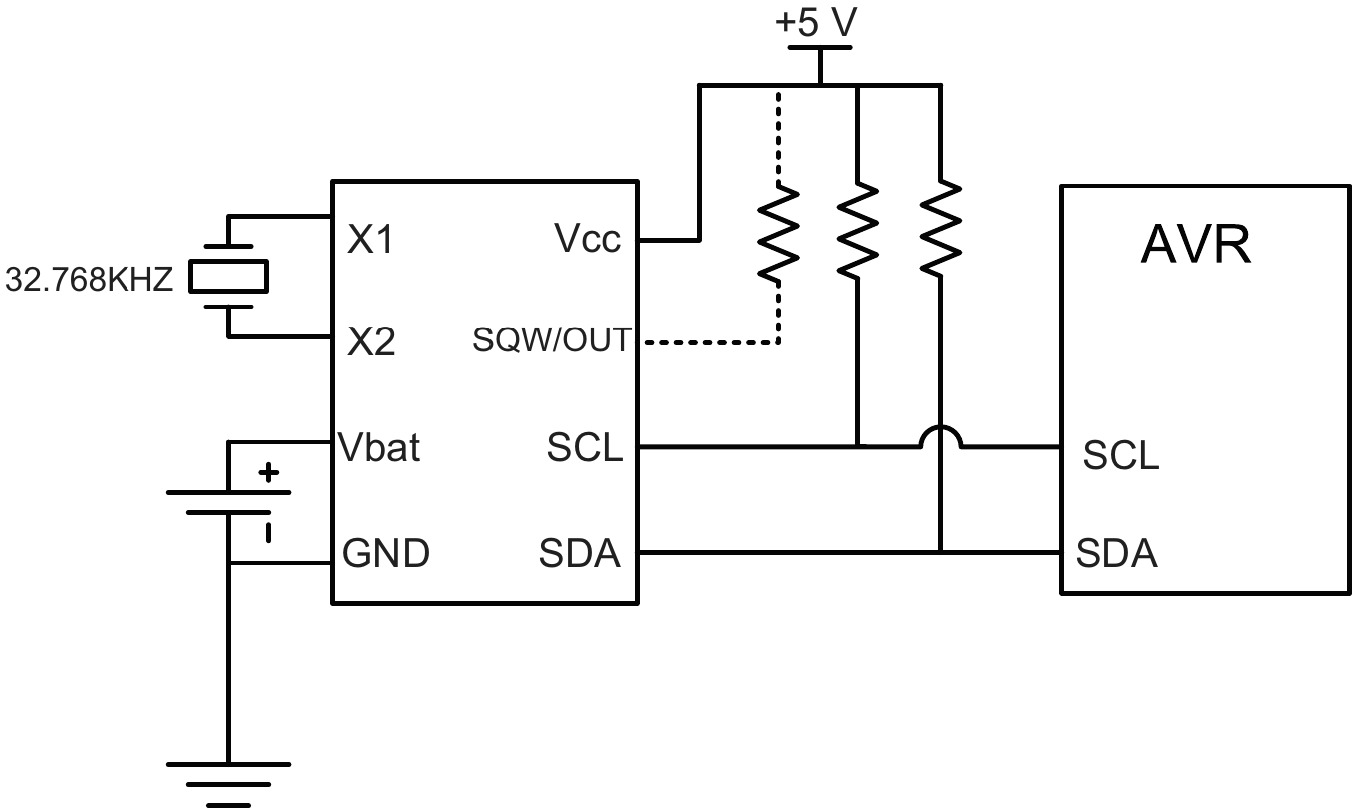
\includegraphics[width=0.85\textwidth]{ds1307-circuit}
        \end{center}

        \framebreak

        \textbf{Address Map of the DS1307:}

        \\~\\

        \scalebox{0.6}{
            \begin{tblr}{
                colspec = {|c|c|c|c|c|c|c|c|c|c|c|},
                hlines, vlines
            }
                \textbf{ADDRESS} & \textbf{Bit7} & \textbf{Bit6} & \textbf{Bit5} & \textbf{Bit4} & \textbf{Bit3} &
                \textbf{Bit2} & \textbf{Bit1} & \textbf{Bit0} & \textbf{FUNCTION} & \textbf{RANGE} \\

                00H & CH & \SetCell[c=3]{c} 10 Seconds & & & \SetCell[c=4]{c} Seconds & & & & Seconds & 00--59 \\
                01H & 0 & \SetCell[c=3]{c} 10 Minutes & & & \SetCell[c=4]{c} Minutes & & & & Minutes & 00--59 \\
                \SetCell[r=2]{c} 02H & \SetCell[r=2]{c} 0 & 12 & 10 Hour & \SetCell[r=2]{c} 10 Hour &
                \SetCell[r=2,c=4]{c} Hours & & & & \SetCell[r=2]{c} Hours & \SetCell[r=2]{c} {1--12 \\ +AM/PM \\ 00--23}
                \\
                & & 24 & PM/AM & & & & & & & \\
                03H & 0 & 0 & 0 & 0 & 0 & \SetCell[c=3]{c} DAY & & & Day & 01--07 \\
                04H & 0 & 0 & \SetCell[c=2]{c} 10 Date & & \SetCell[c=4]{c} Date & & & & Date & 01--31\\
                05H & 0 & 0 & 0 & 10 Month & \SetCell[c=4]{c} Month & & & & Month & 01--12\\
                06H & \SetCell[c=4]{c} 10 Year & & & & \SetCell[c=4]{c} Year & & & & Year & 00--99\\
                07H & OUT & 0 & 0 & SQWE & 0 & 0 & RS1 & RS0 & Control & ---\\
                08H-3FH & \SetCell[c=8]{c} & & & & & & & & RAM 56 x 8 & 00H--FFH\\
            \end{tblr}
        }

        \\~\\

        \begin{itemize}
            \item
            Bit 7 of register 0 is the clock halt (CH) bit. When this bit is set to a 1, the oscillator is disabled.
            When cleared to a 0, the oscillator is enabled.
            \item The byte addresses 0-6 are set aside for the time and date, and
            \textbf{values are stored in BCD format}.
            \item Bit 6 of the hours register is defined as the 12 or 24-hour mode select bit. When high, the 12-hour
            mode is selected. In the 12-hour mode, bit 5 is the AM/PM bit with logic high being PM. In the 24-hour mode,
            bit 5 is the second 10-hour bit.
            \item \textbf{Control Register:} The 07H register is used to control the operation of the SQW/OUT pin.
            \begin{itemize}
                \item \textbf{OUT:}
                This bit controls the output level of the SQW/OUT pin when the square wave output is disabled. If SQWE =
                0, the logic level on the SQW/OUT pin is 1 if OUT = 1 and is 0 if OUT = 0.
                \item \textbf{SQWE (Square Wave Enable):}
                This bit, when set to a logic 1, will enable the oscillator output. The frequency of the square wave
                output depends upon the value of the RS0 and RS1 bits.
                \item \textbf{RS (Rate Select):}
                These bits control the frequency of the square wave output when the square wave
                output has been enabled.
                \begin{tblr}{colspec={|c|c|c|}, hlines, vlines}
                    \textbf{RS1} & \textbf{RS0} & \textbf{SQW Output Frequency} \\
                    0 & 0 & 1Hz \\
                    0 & 1 & 4.096kHz \\
                    1 & 0 & 8.192kHz \\
                    1 & 1 & 32.768kHz \\
                \end{tblr}
            \end{itemize}
        \end{itemize}

        \framebreak

        \textbf{\large Writing to DS1307}\\~\\

        \textbf{Register Pointer:} In DS1307 there is a register pointer that specifies the byte that will be
        accessed in the next read or write command. After each read or write operation,
        the content of the register pointer is automatically incremented. It is useful in
        multibyte read or write.

        \\~\\

        To set the value of the register pointer and write one or more bytes of data to DS1307, we can use the following
        steps:

        \begin{enumerate}
            \item
            To access the DS1307 for a write operation, after sending a START condition, you should transmit the address
            of DS1307 (1001101) followed by 0 to indicate a write operation.
            \item
            The first byte of data in the write operation will set the register pointer.
            \item
            If writing to the set register, we can write one byte at a time (register pointer is incremented after each
            byte).
            \item Transmit a STOP bit condition.
        \end{enumerate}

        \\~\\

        \begin{center}
            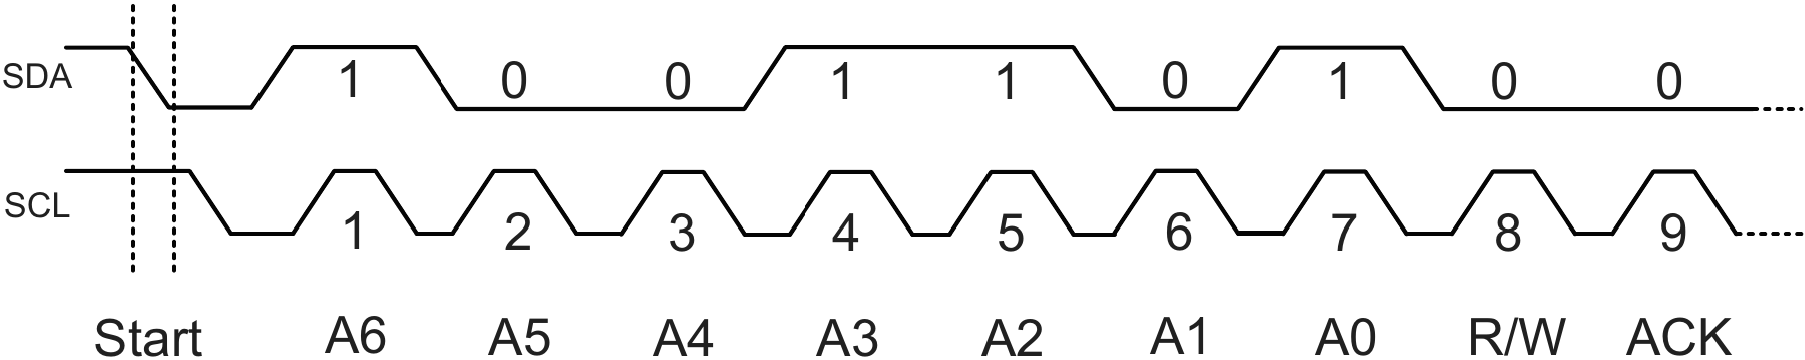
\includegraphics[width=0.9\textwidth]{start-stop-i2c}
        \end{center}

        \\~\\

        \textbf{\large Reading from DS1307}\\~\\

        \begin{enumerate}
            \item Follow steps 1 and 2 of writing procedure and set the address to be read.
            \item After sending a repeated START condition, transmit the address of DS1307 (1001101) follwed by a 1 to
            indicate a read operation. Register pointer will be auto incremeted after transmitting each byte.
            \item Transmit a STOP bit condition.
        \end{enumerate}
    \end{frame}

    \begin{frame}[fragile,allowframebreaks]{Interfacing with AVR Microcontroller}
        \textbf{\large Setting the time in assembly:}
        \\~\\

        \begin{minted}[fontsize=\scriptsize,ignorelexererrors=true]{asm}
.INCLUDE "M32DEF.INC"

    LDI     R21,HIGH(RAMEND)     ;set up stack
    OUT     SPH,R21
    LDI     R21,LOW(RAMEND)
    OUT     SPL,R21

    CALL    I2C_INIT             ;initialize the I2C module

    CALL    I2C_START            ;transmit a START condition
    LDI     R21, 0b11010000      ;SLA (1001101) + W(0)
    CALL    I2C_SEND             ;transmit R21 to I2C bus
    LDI     R21, 0x07            ;set register pointer to 07
    CALL    I2C_SEND             ;to access the control register
    LDI     R21, 0x00            ;set control register = 0
    CALL    I2C_SEND             ;transmit R21 to I2C bus
    CALL    I2C_STOP             ;transmit a STOP condition

    CALL    DELAY

    CALL    I2C_START            ;transmit a START condition
    LDI     R21, 0b11010000      ;SLA (1001101) + W(0)
    CALL    I2C_SEND             ;transmit R21 to I2C bus
    LDI     R21, 0x00            ;set register pointer to 0
    CALL    I2C_SEND             ;transmit R21 to I2C bus
    LDI     R21, 0x55            ;set seconds to 0x55 = 55 BCD
    CALL    I2C_SEND             ;transmit R21 to I2C bus
    LDI     R21, 0x58            ;set minutes to 0x58 = 58 BCD
    CALL    I2C_SEND             ;transmit R21 to I2C bus
    LDI     R21, 0b00010110      ;hour = 16 in 24 hours mode
    CALL    I2C_SEND             ;transmit R21 to I2C bus
    CALL    I2C_STOP             ;transmit a STOP condition

HERE:
    RJMP    HERE                 ;wait here forever

;********************************************************
I2C_INIT:
    LDI     R21, 0
    OUT     TWSR,R21             ;set prescaler bits to zero
    LDI     R21, 0x47
    OUT     TWBR,R21             ;SCL freq. is 50k for 8 MHz XTAL
    LDI     R21, (1<<TWEN)
    OUT     TWCR,R21             ;enable the TWI
    RET

;********************************************************
I2C_START:
    LDI     R21, (1<<TWINT)|(1<<TWSTA)|(1<<TWEN)
    OUT     TWCR,R21             ;transmit a START condition
W1: IN      R21, TWCR            ;read control register into R21
    SBRS    R21, TWINT           ;mask the interrupt flag
    RJMP    W1                   ;jump to W1 if TWINT is 1
    RET

;********************************************************
I2C_SEND:
    OUT     TWDR, R21            ;move SLA+W into TWDR
    LDI     R21, (1<<TWINT)|(1<<TWEN)
    OUT     TWCR,R21             ;configure TWCR to send TWDR
W2: IN      R21, TWCR            ;read control register into R21
    SBRS    R21, TWINT           ;mask the interrupt flag
    RJMP    W2                   ;jump to W2 if TWINT is 1
    RET

;********************************************************
I2C_STOP:
    LDI     R21, (1<<TWINT)|(1<<TWSTO)|(1<<TWEN)
    OUT     TWCR,R21             ;transmit STOP condition
W3: IN      R21, TWCR            ;read control register into R21
    SBRS    R21, TWSTO           ;mask the interrupt flag
    RJMP    W3                   ;jump to W3 if TWINT is 1
    RET

;********************************************************
DELAY:
    LDI     R22, 0xFF
A1: DEC     R22                  ;transmit STOP condition
    NOP
    BRNE    A1
    RET
        \end{minted}
    \end{frame}
\end{document}